\documentclass[main_estudante.tex]{subfiles}

\begin{document}

\chapter{Equação de retas e circunferências}

\section{Questões diagnósticas}

\begin{diagnostico}
Considere os pontos $P=(1;3)$ e $Q=(-1;-1)$.
\begin{enumerate}[a)]
\item Obtenha a equação da reta que passa pelos dois pontos.
\item Dê a equação de uma reta diferente e paralela à encontrada no item a.
\end{enumerate}
\end{diagnostico}

\begin{diagnostico}
Considere as retas dadas pelas equações $2y+2x-1=0$ e $y-4x-3=0$.
\begin{enumerate}[a)]
\item Obtenha o ponto de intersecção entre as duas retas.
\item Represente as retas em um plano cartesiano.
\end{enumerate}
\end{diagnostico}

\section{Gabarito}

\textbf{Questão 1:} a) $y=2x+1$, b) No caso de uma equação na forma reduzida, basta tem coeficiente angular igual a $2$ e coeficiente linear diferente de $-1$. No caso de a equação estar em outro formato, é necessaŕio converter para a forma reduzida.

\textbf{Questão 2:} a) $(-1/2;1)$. b) É importante apenas que as retas se cruzem em um ponto coerente com a resposta anterior, uma seja crescente e a outra decrescente.

\section{Quadro de orientação}

\begin{center}
 \begin{tabular}{|c c c |c|} 
 \hline
 1A & 1B & 2A e 2B & Onde começar\\
 \hline
 C & E & E & Questão 2 \\ 
 \hline
 C & C & E & Questão 6 \\ 
 \hline
 C & C & C & Questão 7 \\ 
 \hline
\end{tabular}
\end{center}

\section{Comentários iniciais}

Esse capítulo trata da equação da reta e da circunfência (no plano) em três formatos diferentes: reduzida ($y=ax+b$ e $(x-x_0)^2+(y-y_0)^2=r^2$), geral ($ax+bc+c=0$ e $ax^2+bx+cy^2+ey+f=0$) e paramétrica.

Para além desses tópicos específicos, este capítulo também pretende tocar em alguns aspectos que serão importantes no tratamento de outros objetos em Geometria Analítica, como vetor normal de um plano (ao tratar da equação geral da reta), identificação de cônicas (ao tratar da forma geral da circunferência) e equações paramétricas em geral (ao tratar desses dois casos específicos). Esses aspectos são abordados de maneira indireta, mas são bastante importantes.

\section{Questões comentadas}

\begin{questao}
Considere os pontos $P=(1;1)$ e $Q=(3;5)$.
\begin{enumerate}[a)]
\item Marque os dois pontos em um eixo cartesiano.
\item Trace a reta que passa pelos dois pontos.
\item Avaliando visualmente, você diria que quais dos seguintes pontos estão sobre a reta: $A=(-1;2)$,$B=(4;4)$, $C=(2;3)$, $D=(-1;-3)$?
\item Avaliando visualmente, em quais pontos essa reta parece cortar os eixos $X$ e $Y$?
\end{enumerate}
\end{questao}

Essa questão é bem introdutória e só será resolvida pelos estudantes que não acertaram nenhuma questão na avaliação diagnóstica. Nossa intenção é começar com algo puramente visual e introduzir elementos gradativamente. Dificuldades nessa questão podem significar uma defasagem bastante grande em conteúdos bastante básicos. Não tenha pressa e deixe que os estudantes com dificuldade resolvam lentamente as questões vindouras.

O ponto $D$ pode ser dúbio em uma análise visual, como mostrado no gabarito, e isso reforça a vantagem da expressão agébrica.

\begin{questao}
Obtenha a equação da reta que passa pelos pontos $P=(1;1)$ e $Q=(3;5)$.
\end{questao}

A questão acima ainda é bastante básica considerando o ponto do semestre em que esse capítulo está sendo usado. SE algum estudante estiver com dificuldade, crie algumas variações escolhendo pares de pontos e peça que resolvam por dois métodos diferentes: 1) obtendo o coeficiente angular e então o coeficiente linear e 2) usando a forma $y=ax+b$ e resolvendo o sistema para $a$ e $b$.

\begin{questao}
Considere a reta dada pela equação $y=2x-1$, responda:
\begin{enumerate}[a)]
\item Qual é o ponto de coordenada $X$ igual a $10$ que pertence a essa reta?E de coordenada $Y$ igual a $-3$?
\item Em que pontos ela corta os eixos $X$ e $Y$?
\item Quais dos pontos $A=(-1;2)$,$B=(4;4)$, $C=(2;3)$ e $D=(-1;-3)$ pertencem a ela? 
\item Dê as coordenadas de um ponto do quarto quadrante (valores de $X$ positivos e de $Y$ negativos) que pertença à reta.
\end{enumerate} 
\end{questao}

O objetivo dessa questão é contrapor a valiação visual da primeira questão com a avaliação algébrica (e você pode explicitar isso) e certificar de que os estudantes estão familiarizados com conceitos e propriedades bastante elementares, como intersecção com os eixos e quadrantes.

Em caso de dificuldades, gere variações da questão criando outras equações de reta na forma reduzida e propondo questões similares.

\begin{questao}
Usando um único plano cartesiano, esboce a retas dadas pelas equações: $y=x+1$, $y=-2x-4$, $y=\frac{x}{2}$ e $y=\frac{x}{2}-1$.
\end{questao}

Mais do que precisão, é importante que os estudantes acertem as diferenças e semelhanças entre as representações: qual é mais verticalizada? Qual cruza o eixo Y mais abaixo?

\begin{questao}
Dê a equação de uma reta paralela à reta $y=2x-1$.
\end{questao}

Espera-se que aqui os estudantes sejam capazes de uma generalização simples envolvendo coeficiente angular. Você pode pedir a eles que escrevam essa propriedade como um complemento a essa questão.

\begin{questao}
Dada a reta de equação $4y+6x-4=0$, faça o que se pede:
\begin{enumerate}[a)]
\item Determine os pontos em que ela corta os eixos $X$ e $Y$.
\item Esboce a reta em um plano cartesino.
\end{enumerate} 
\end{questao}

\begin{questao}
Esboce o gráfico das retas com equações iguais a $x-5=0$, $y+1=0$, $2x+1=0$ e $y=0$.
\end{questao}

Questões simples para introduzir a forma geral. Nenhuma dificuldade é esperada.

\begin{questao}
Em relação à reta acima:
\begin{enumerate}[a)]
\item Use o quadriculado para traçar um vetor perpendicular à reta a partir do ponto $(0;2)$. Sugestão: trace um vetor que termine em um dos vértices do quadriculado.
\item Quais são as dimensões desse vetor?
\end{enumerate} 
\end{questao}

Essa propriedade é muito utilizada em Geometria Analítica e raramente abordada no Ensino Médio. Apesar de não parecer tão poderosa em duas dimensões, ela facilita muitos cálculos no espaço. Inclusive, essa propriedade está relacionada com a fórmula ara obtenção do coeficiente angular de uma reta perpendicular a uma dada no plano.

\begin{questao}
Seja $\overrightarrow{V}=\binom{1}{2}$ e $P=(1;1)$.
\begin{enumerate}[a)]
\item Marque o ponto $P$ no quadriculado abaixo e o vetor $\overrightarrow{V}$ começando em $P$.

\begin{figure}[h]
\centering
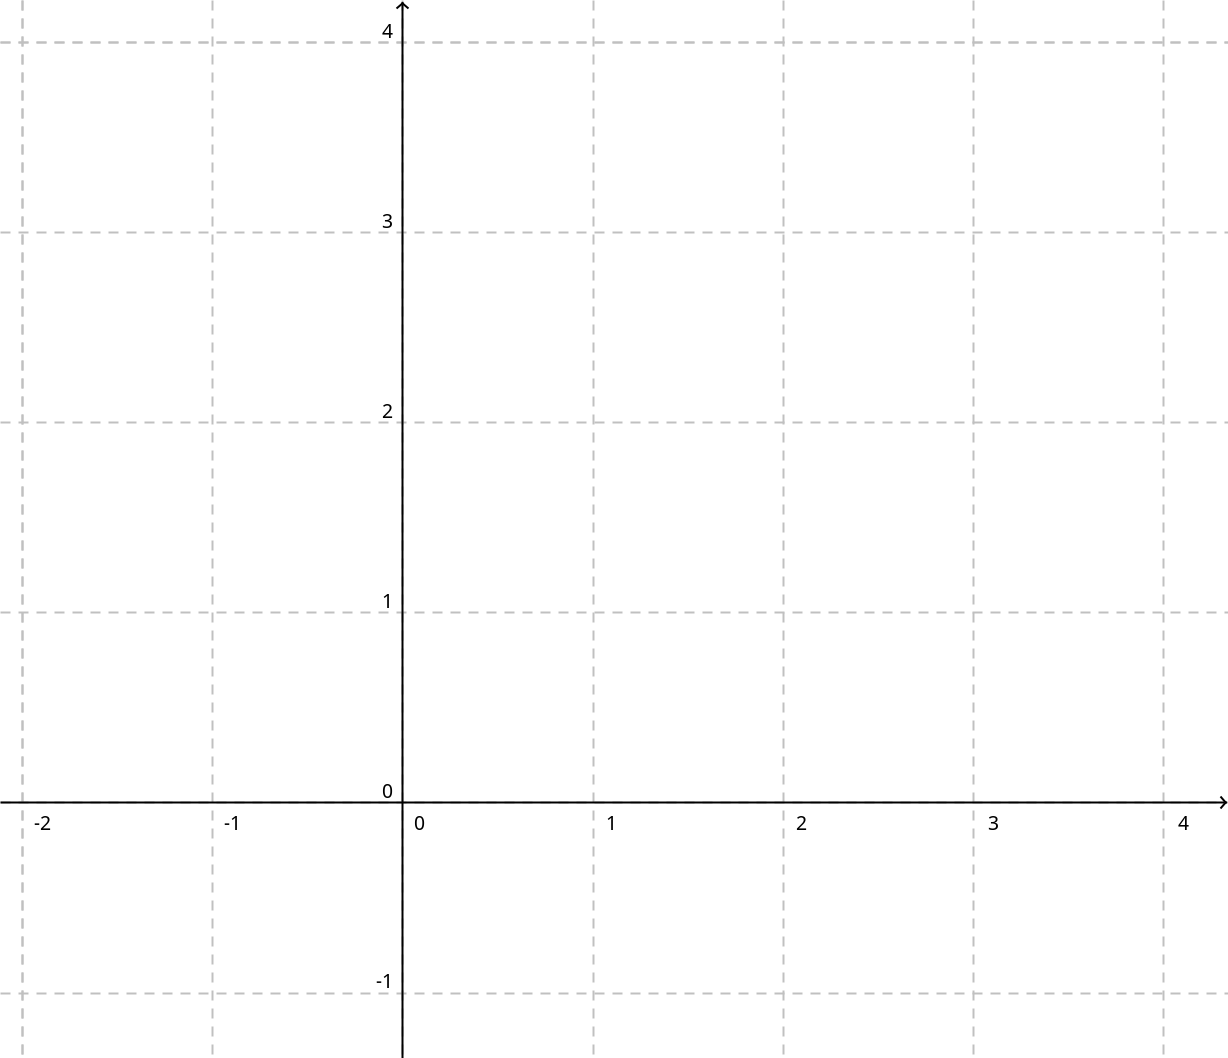
\includegraphics[width=0.7\textwidth]{./img/c6q9.png}
\end{figure}

\item Visualmente, trace uma reta que passa por $P$ e é perpendicular a $\overrightarrow{V}$.
\item Obtenha a equação dessa reta.
\item Obtenha a equação de uma nova reta que passa pelo ponto $Q=(3;2)$ e tem vetor normal igual a $\overrightarrow{U}=\binom{5}{-1}$.
\end{enumerate}
\end{questao}

Essa questão soa incomum no contexto do Ensino Médio, mas para planos no espaço o vetor normal é uma referência de direção muito mais eficiente do que as inclinações do plano em relação aos eixos, por isso ela foi incluída aqui. A intenção é fazer com que o estudante perceba que dependendo das informações disponíveis, a forma geral pode ser mais conveniente do que a reduzida.

\begin{reflita}
 Compare com seus colegas o método que você utilizou pra resolver o último item da questão acima e descreva com suas palavras o método que lhe parece o melhor para resolvê-la quando a informação dada é um ponto e o vetor normal da reta.
\end{reflita}

O último item da questão anterior pode ser resolvido usando apenas a forma geral (método novo, mas mais simples) ou passando-se pela forma reduzida (método familiar, mas mais longo). A intenção da questão continua sendo reforçar as vantagens e desvantagens de cada forma.

\begin{questao}
Em relação à reta dada pela equação $(x,y)=(2t-1;t+3)$, faça o que se pede.
\begin{enumerate}[a)]
\item Obtenha as coordenadas dos pontos para $t=0$, $t=2$ e $t=-1$.
\item Marque esses pontos no plano cartesiano abaixo e confirme que eles pertencem a uma mesma reta, ou seja, estão alinhados.

\begin{figure}[h]
\centering
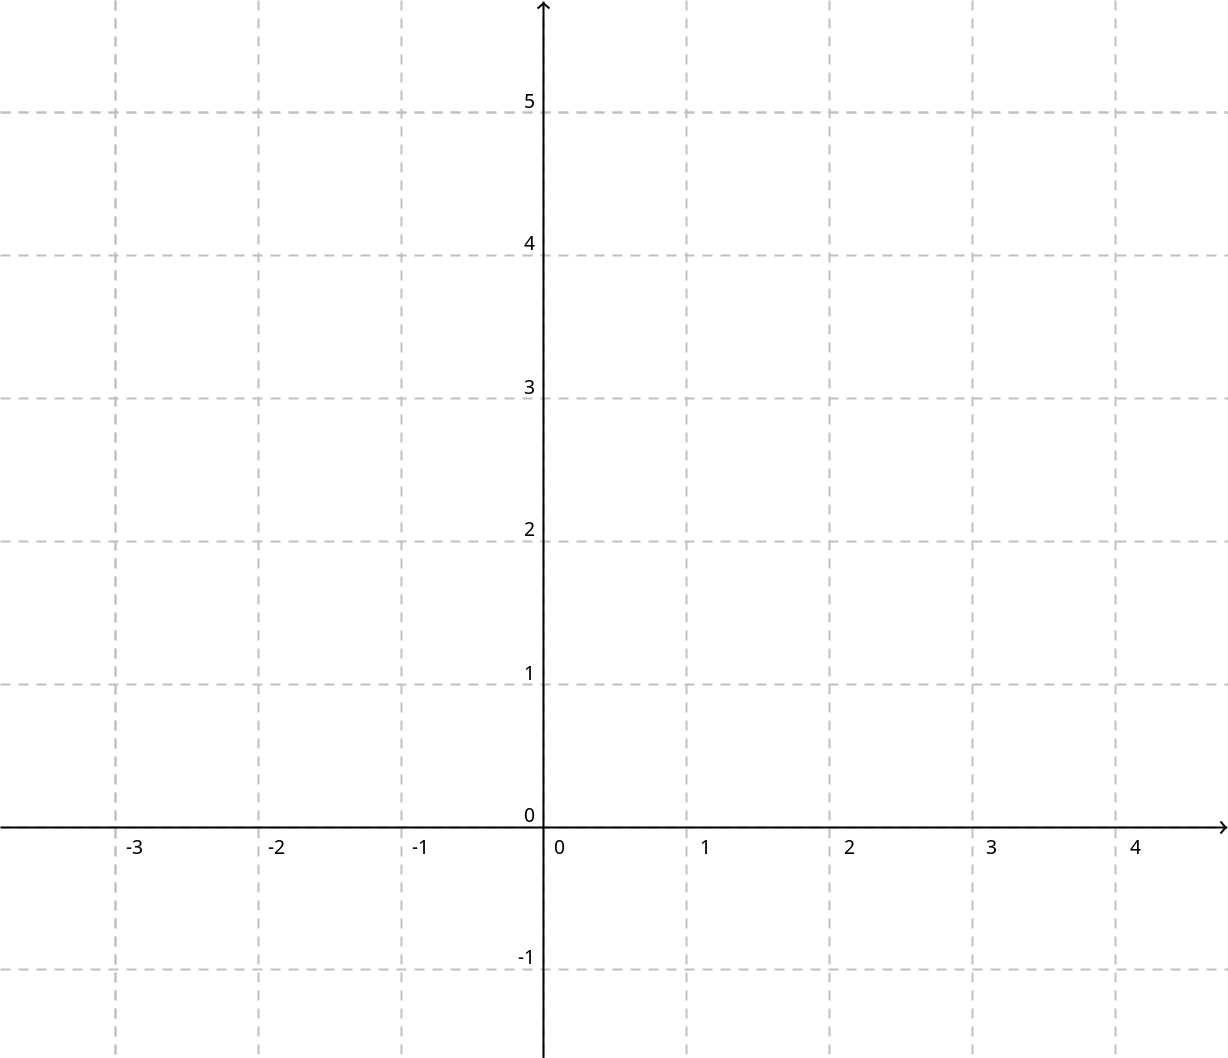
\includegraphics[width=0.7\textwidth]{./img/c6q10.png}
\end{figure}

\item Determine para quais valores de $t$ essa reta cruza os eixos $X$ e $Y$.
\end{enumerate} 
\end{questao}

Neste ponto a forma paramétrica é introduzida. Apesar de não oferecer tantas vantagens para retas e planos, a forma paramétrica não é muito discutida no Ensino Médio e introduzi-la com um objeto simples como retas no plano pode facilitar o seu uso para curvas mais complexas. Nenhuma dificuldade específica é esperada.

\begin{questao}
Considere os pontos $P=(1;1)$ e $Q=(3;5)$.
\begin{enumerate}[a)]
\item Marque esses pontos em um plano cartesiano e trace a reta que passa por eles.
\item Obtenha a equação dessa reta na forma reduzida (suportamente a mais simples para o caso em que dois pontos são dados).
\item Obtenha a equação na forma geral manipulando algebricamente a equação obtida no item anterior.
\item Use a equação na forma geral para obter o vetor normal e trace-o no mesmo plano cartesiano.
\item Obtenha uma equação paramétrca que represente essa mesma reta usando as ideias de ponto inicial e direção da reta.
\end{enumerate} 
\end{questao}

Essa questão conclui a parte sobre retas, reunindo todas as formas vistas e sugerindo a conversão entre elas. A última delas deve ser a mais desafiadora por ser nova aos estudantes. Nossa sugestão é que se use uma abordagem intuitiva que começa com a escolha visual de um ponto inicial e depois de um vetor de direção e então a montagem da reta. A questão seguinte, do tipo Reflita, deve promover um pouco de discussão sobre essas escolhas.

\begin{reflita}
Compare com seus colegas para ver se todos obtiveram as mesmas respostas para os itens b, c e e. Em quais desses itens é possível obter respostas diferentes corretas? 
\end{reflita}

A forma reduzida é única para cada reta (não vertical), mas a forma geral e a paramétrica admitem diversas equações para uma mesma reta (do ponto de vista geométrico). A forma geral pode ser multiplicada por constantes gerando novas equações para uma mesma reta. A forma paramétrica pode ter diferentes pontos iniciais e diferentes vetores direção (múltiplos um do outro). Pode-se argumentar que diferentes pontos iniciais e diferentes vetores de direção geram retas diferentes (no contexto da Física estaríamos falando de um mesmo trajeto iniciado em locais e com velocidades diferentes), mas a representação visual delas é a mesma.

\begin{questao}
Use a equação dada acima para responder as questões abaixo.
\begin{enumerate}[a)]
\item Qual é a equação da circunferência com centro em $(2;1)$ e raio 3? 
\item Qual é a equação da circunferência com centro na origem e raio 1?
\item Qual é o centro e raio da circunferência dada pela equação $(x-1)^2+(y+3)^2=4$?
\end{enumerate} 
\end{questao}

Essa é a primeira questão sobre circunferências e não deve gerar dificuldades.

\begin{questao}
Obtenha o raio e centro da circunferência dada pela equação $x^2+2x+y^2-8y+13=0$
\end{questao}

Essa questão é substancialmente mais difícil do que a anterior, mas pode ser resolvida do mesmo modo que o exemplo discutido no texto foi. Insista que os estudantes leiam o texto que antecede a questão antes de resolvê-la. Apesar de estarmos explorando apenas a circunferência, esse tipo de questão é comum em Geometria Analítica no contexto mais geral das curvas cônicas, portanto, não tenha pressa e certifique-se de que os estduantes entenderam o método ao invés de terem criado algum tipo de procedimento rígido para ele.

\begin{questao}
Visando praticar um pouco mais o uso da forma geral de uma circunferência, faça o que se pede a seguir:
\begin{enumerate}[a)]
\item Escolha o centro e raio de uma circunferência, escreva a sua forma reduzida e desenvolva-a de modo a obter a sua forma geral.
\item Passe apenas a forma geral para um colega e obtenha o centro e raio da circunferência por trás da forma geral que ele te passou.
\item Cheque se ambos acertaram a questão.
\end{enumerate} 
\end{questao}

A questão visa apenas promover um pouco de prática com a forma geral da circunferência usando uma dinâmica um pouco diferente para trabalho em duplas.

\begin{questao}
Considerando a figura acima:
\begin{enumerate}[a)]
\item Como a coordenada $X$ do ponto $P$ pode ser obtido em termos do ângulo $\alpha$?
\item Como a coordenada $Y$ do ponto $P$ pode ser obtido em termos do ângulo $\alpha$?
\item Se considerarmos $\alpha$ como parâmetro, como ficaria a equação paramétrica da circunferência mostrada acima?
\end{enumerate} 
\end{questao}

Neste ponto a forma paramétrica da circunferência é introduzida. Apesar de não usual, essa forma ainda é bastante simples e não esperamos dificuldades. Esse equação especificamente não aparece na ementa de Geometria Analítica, mas a sua simplicidade facilita a exploração de equações paramétricas como um todo. Esse é o objetivo do bloco de questões a seguir: criar alguma familiaridade com equações paramétricas simples. 

Fique atento com as questões anteriores, pois elas tem um caráter menos diretivo e mais aberto. Os estudantes podem se sentir perdidos por terem menos orientações explícitas sobre como proceder. Evite ser diretivo e foque em sugestões mais genéricas como: que tal tentar alterar um pouco a equação que você já conhece? Marque alguns pontos para essa equação e veja se você nota algo.

\begin{questao}
Você obteve a equação $(x;y)=(\cos(t);\sin(t))$ para a circunferência de centro na origem e raio $1$ na questão anterior. Quais são as semelhanças e diferenças entre ela e a curva obtida pela equação $(x;y)=(\sint);\cos(t))$?
\end{questao}

A única diferença se refere ao ponto em que a curva começa ($t=0$).

\begin{questao}
Esboce a curva gerada pela equação paramétrica $(x;y)=(3\cos(t);4\sin(t))$. Como você descreveria essa curva?
\end{questao}

Trata-se de uma elipse. Note que a aparência da curva não é suficiente para afirmar que de fato se trata de uma elipse (seria necessário demonstrar que a curva atente a alguma definição formal de elipse).

\begin{questao}
Qual deve ser a equação paramétrica da circunferência com centro na origem e raio igual a $3$?
\end{questao}

\begin{questao}
Qual deve ser a equação paramétrica da circunferência de raio $1$ e centro em $(2;3)$?
\end{questao}

As duas questões acima de certa forma adiantam o conteúdo do próximo capítulo (transformação de gráficos). Incentive os estudantes a fazerem tentativas e validarem essas tentativas através de marcação de pontos em um plano cartesiano.

\section{Rumo ao livro texto}

Diferentemente dos capítulos anteriores, a proposta aqui é que o estudante leia uma seçã do livro texto. Essa seção parte de propriedades no plano para discutir retas e planos no espaço. Esperamos que as questões resolvidas e discutidas ao longo do texto facilitem a compreensão do livro-texto.

\section{Gabarito}

\noindent\textbf{Questão 1:} 

\begin{figure}[h]
\centering
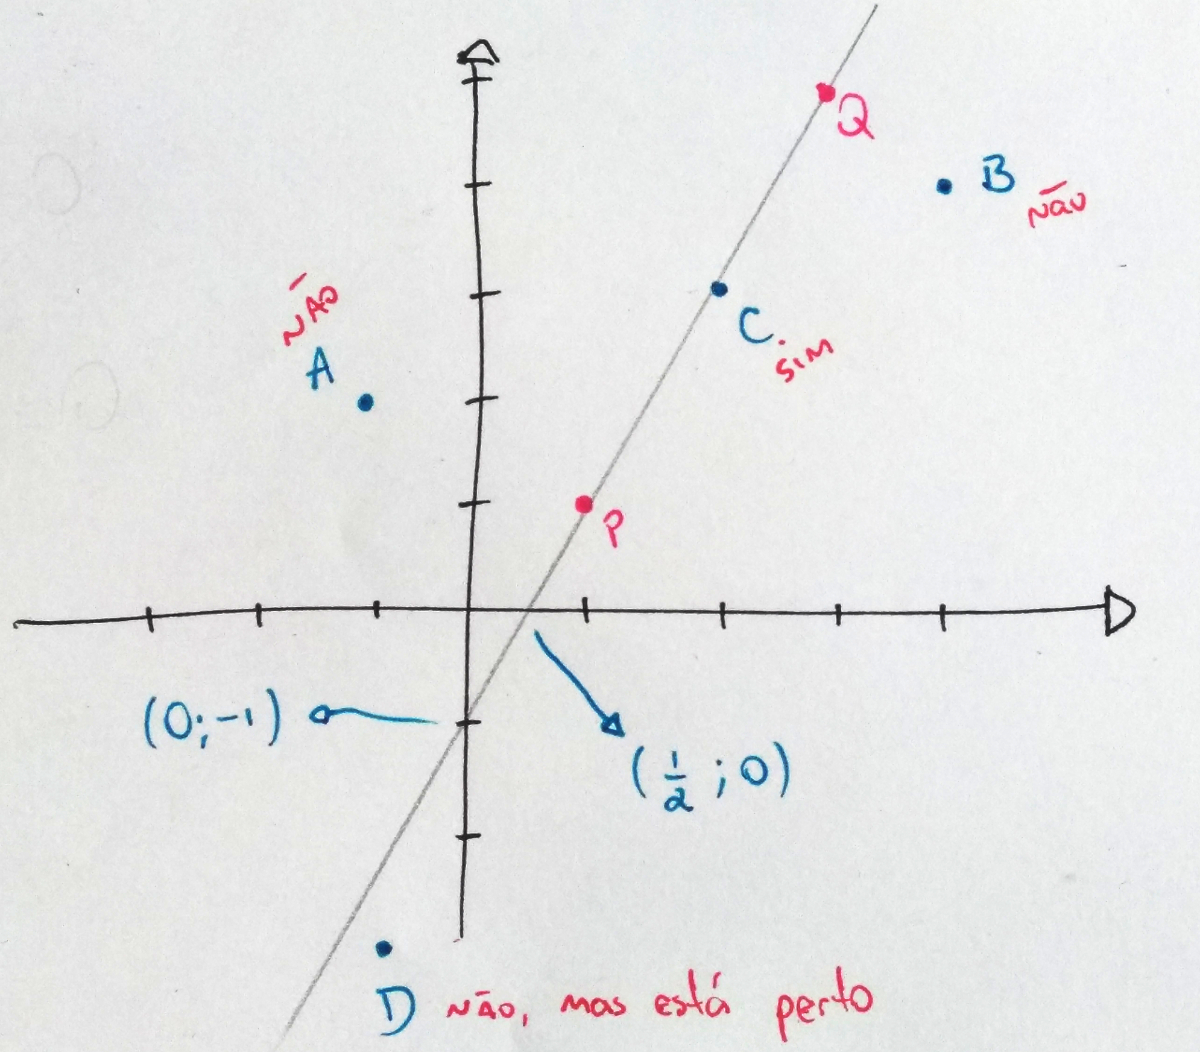
\includegraphics[width=0.5\textwidth]{./img/c6g1.jpg}
\end{figure}

\noindent\textbf{Questão 2:} a) $y=2x-1$.

\noindent\textbf{Questão 3:} a) $(10;19)$ e $(-1;-3)$, b) $(1/2;0)$ e $(0;-1)$, c) Apenas $C$ e $D$.

\noindent\textbf{Questão 4:} 

\begin{figure}[h]
\centering
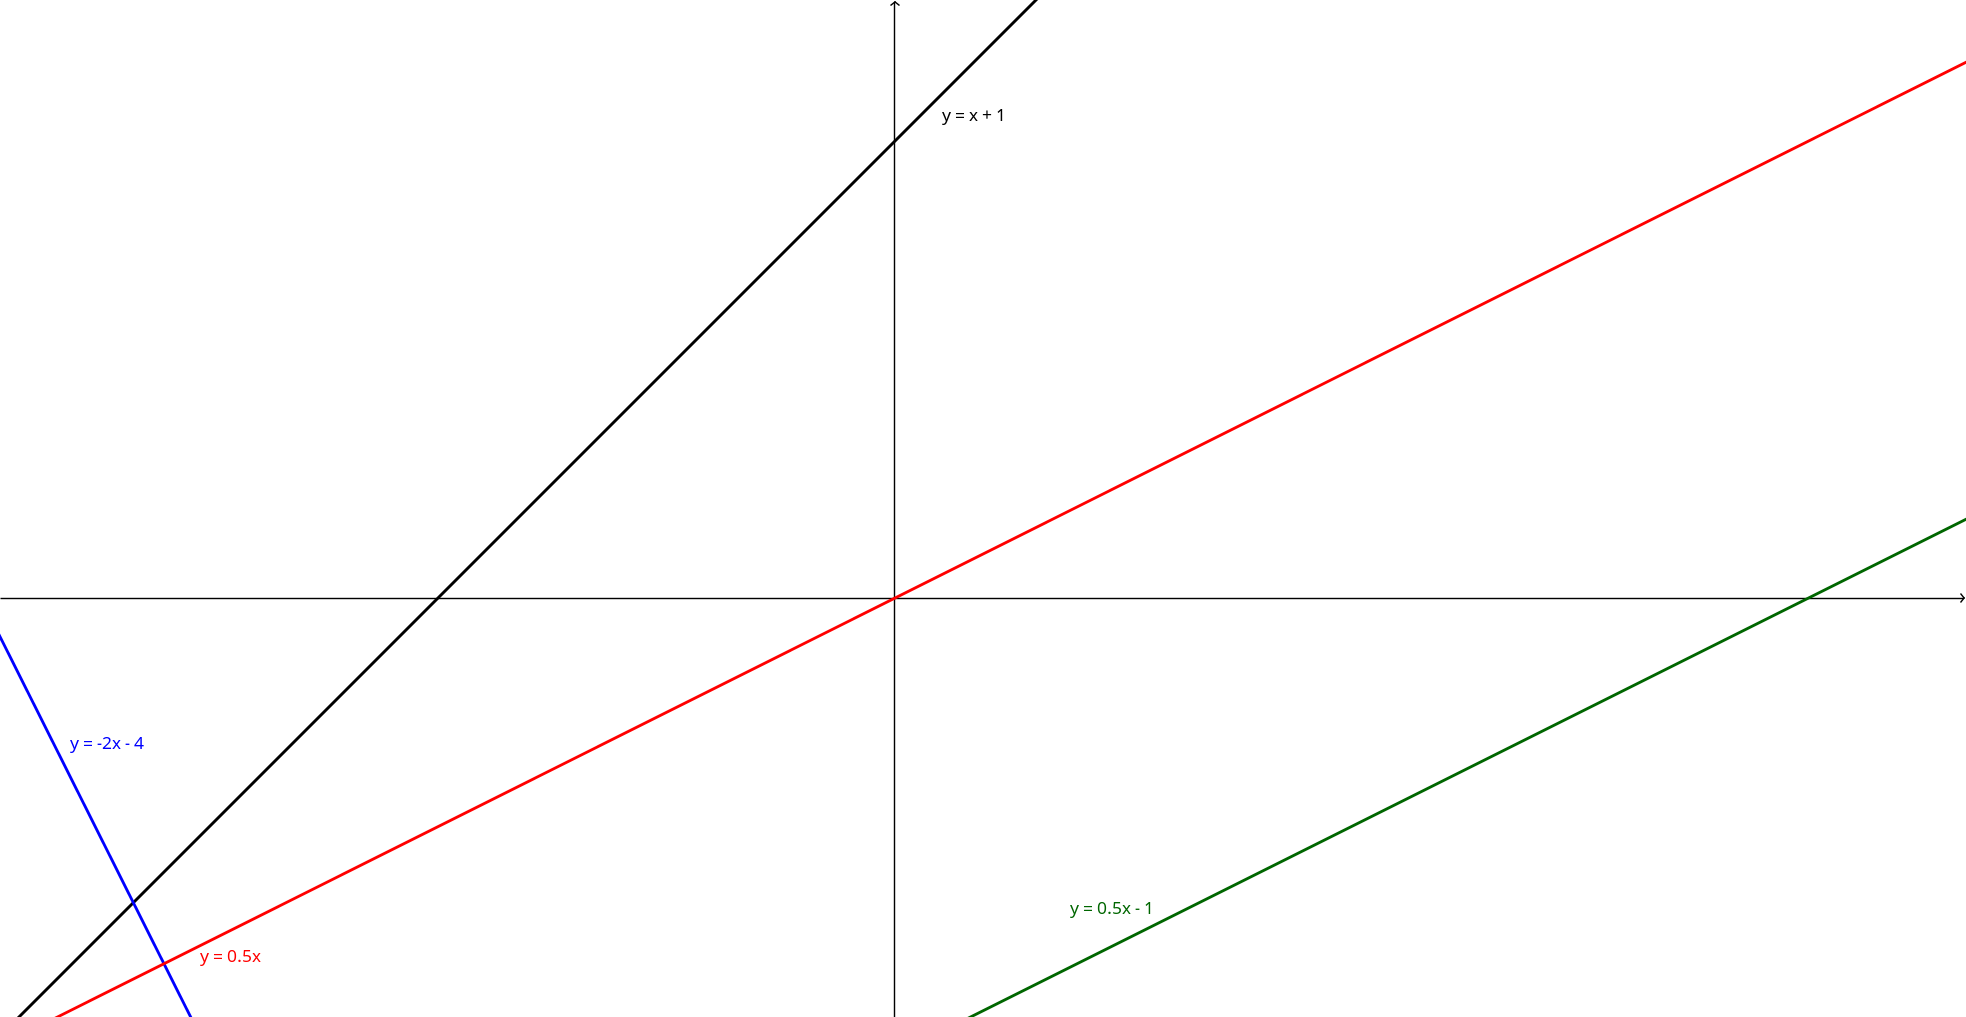
\includegraphics[width=0.5\textwidth]{./img/c6g4.png}
\end{figure}

\noindent\textbf{Questão 5:} $y=2x-2$, por exemplo.

\noindent\textbf{Questão 6:} a) $(2/3;0)$ e $(0;1)$, b) cheque com seu tutor ou colega.

\noindent\textbf{Questão 7:} 

\begin{figure}[h]
\centering
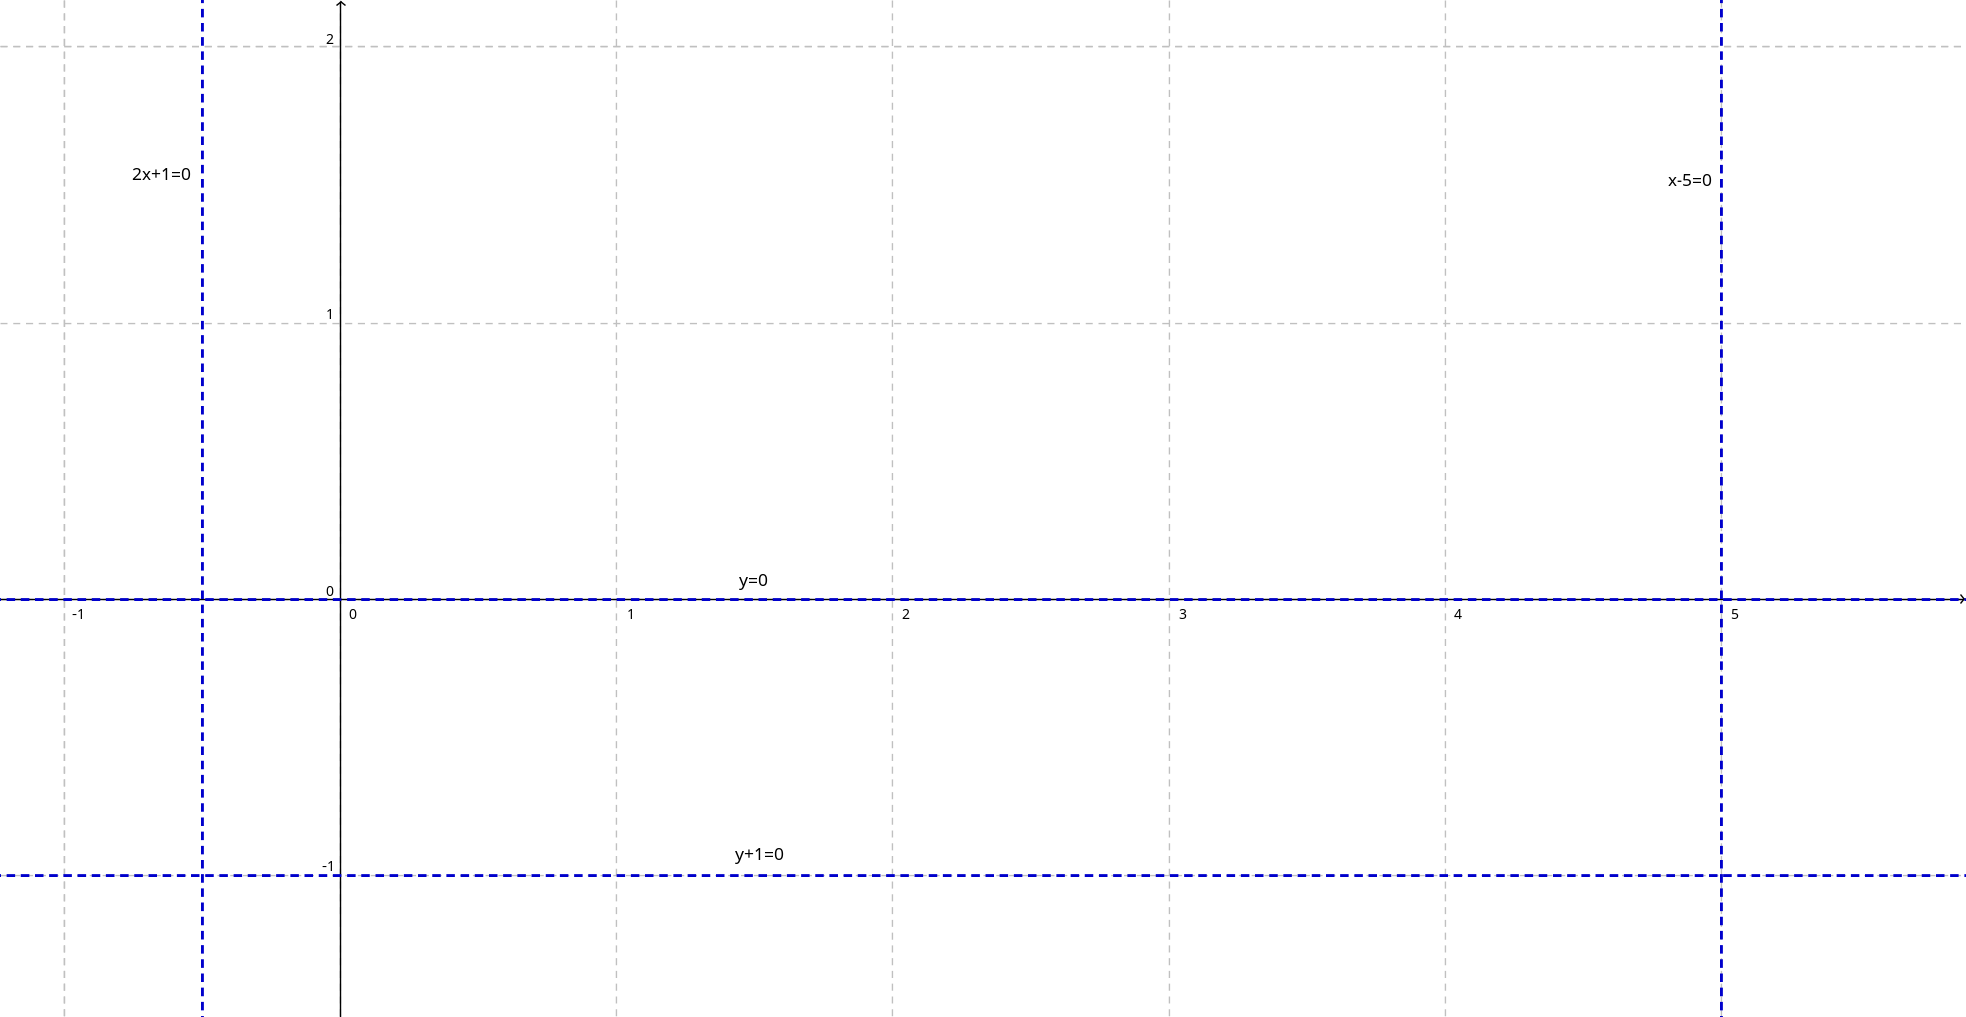
\includegraphics[width=0.5\textwidth]{./img/c6g7.png}
\end{figure}

\noindent\textbf{Questão 8:} b) $(-1;2)$ é uma possibilidade correta.

\noindent\textbf{Questão 9:} a) e b) abaixo, c)$2y+x-3=0$, d) $-y+5x-13=0$.

\begin{figure}[h]
\centering
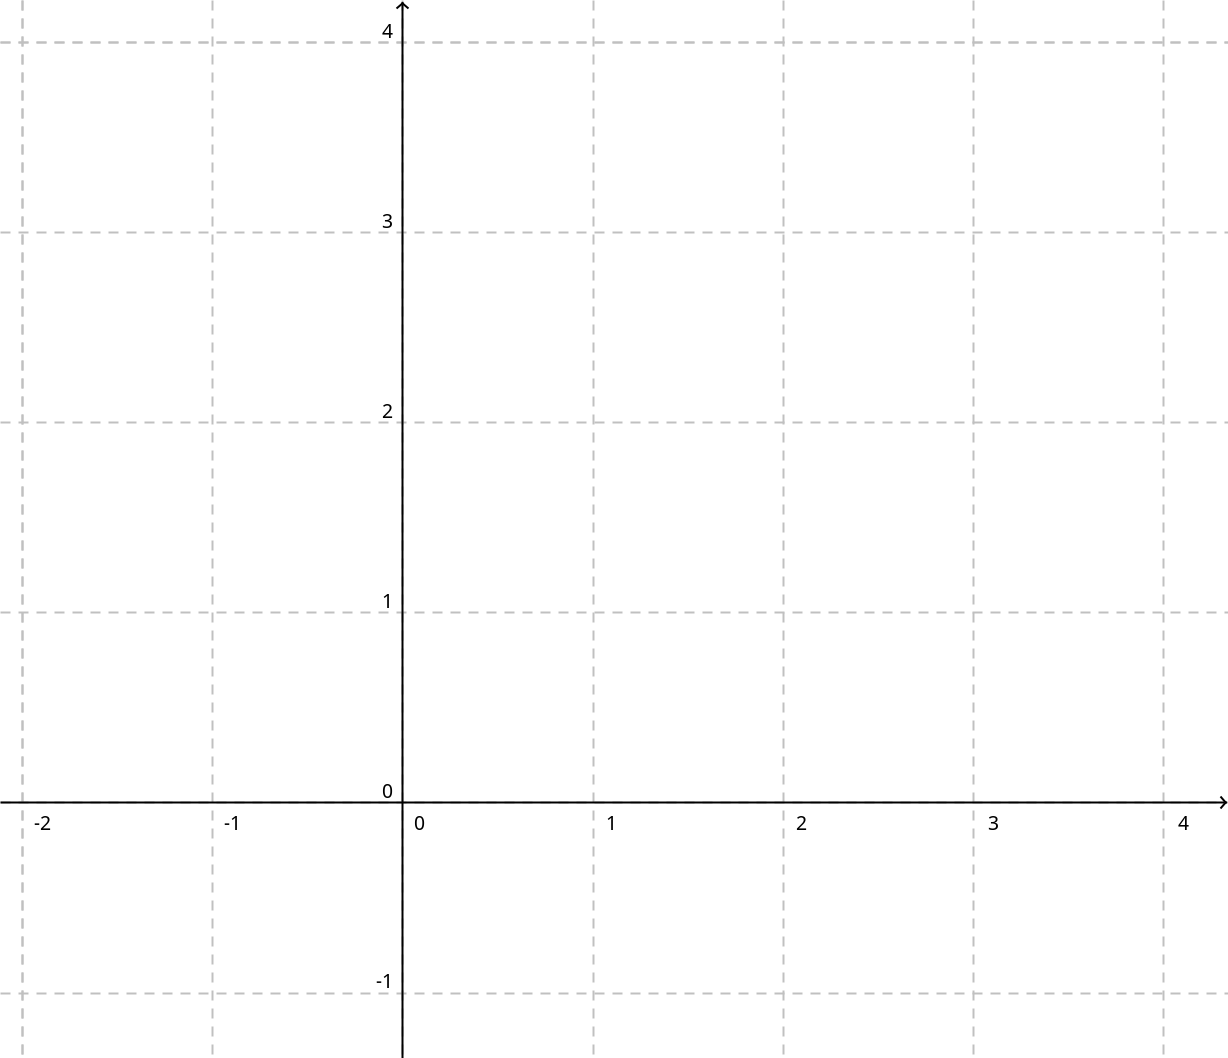
\includegraphics[width=0.7\textwidth]{./img/c6q9.png}
\end{figure}

\noindent\textbf{Questão 10:} a) $(-1;3)$, $(3;5)$ e $(-3;2)$, c) $t=-3$ e $t=1/2$.

\noindent\textbf{Questão 11:} b) $y=2x-1$, c) $y-2x+1=0$, d) $\overrightarrow{V}=(-2;1)$, e) $(x;y)=(1;1)+(2;4) \cdot t$.

\noindent\textbf{Questão 12:} a) $(x-2)^2+(y-1)^2=3^2$, b) $x^2+y^2=1$, c) $(1;-3)$ e $r=2$.

\noindent\textbf{Questão 13:} $(-1;+4)$ e $r=2$.

\noindent\textbf{Questão 15:} a) $x=\cos(\alpha)$, b) $y=\sin(\alpha)$,  c) $(x;y)=(\cos(\alpha);\sin(\alpha))$.

\section{Questões adicionais}

Ao final da seção sobre retas, você pode propor questões envolvendo o ponto de intersecção entre pares de retas.

\begin{adicional}
Obtenha o ponto de intersecção entre as retas dadas abaixo:
\begin{enumerate}[a)]
\item $y=3x-2$ e $5y-6x+1=0$.
\item $2x+3y-5=0$ e $(t-1;-2t+3)$.
\item $(2t;-t)$ e $(t+2;3t-1)$.
\end{enumerate} 
\end{adicional}

O primeiro item é simples (resposta: $(1;1)$). O segundo pode ser resolvido substituindo as expressões pra $x$ e $y$ da forma paramétrica na forma geral (resposta: $(-1/2;2)$). O terceiro exige um passo que pode não ser intuitivo: o valor de $t$ nas duas representações não precisa ser igual. Use $t_1$ e $t_2$ e iguale as coordenadas, caindo em um sistema (resposta: $(2;-1)$).

A próxima questão segue na direção da identificação de cônicas dadas na forma geral. Trata-se da hipérbole de equação reduzida $(x-3)^2-(y+2)^2=1$.

\begin{adicional}
Sabendo que a expressão geral $x^2-y^2-6x-4y+4=0$ veio de uma expressão reduzida do tipo $(x-a)^2-(y-b)^2=c$, obtenha a expressão reduzida original.
\end{adicional}

\end{document}
